\documentclass[a4paper,12pt]{article}

\usepackage[T2A]{fontenc}			
\usepackage[utf8]{inputenc}			
\usepackage[english,russian]{babel}	

\usepackage[
bookmarks=true, colorlinks=true, unicode=true,
urlcolor=black,linkcolor=black, anchorcolor=black,
citecolor=black, menucolor=black, filecolor=black,
]{hyperref}

\usepackage{color}
\usepackage{caption}
\DeclareCaptionFont{white}{\color{black}}
\DeclareCaptionFormat{listing}{\colorbox{white}{\parbox{\textwidth}{#1#2#3}}}
\captionsetup[lstlisting]{format=listing,labelfont=white,textfont=white}

\usepackage{amsmath,amsfonts,amssymb,amsthm,mathtools} 
\usepackage{wasysym}

\usepackage{graphicx}
%\usepackage[cache=false]{minted}
\usepackage{cmap}
\usepackage{indentfirst}

\usepackage{listings} 
\usepackage{fancyvrb}

\usepackage{geometry}
\geometry{left=2cm}
\geometry{right=1.5cm}
\geometry{top=1cm}
\geometry{bottom=2cm}

\setlength{\parindent}{5ex}
\setlength{\parskip}{0.5em}

\usepackage{pgfplots}
\usetikzlibrary{datavisualization}
\usetikzlibrary{datavisualization.formats.functions}

\begin{document}
	\lstset{ %
		language=C,                 % выбор языка для подсветки (здесь это С)
		basicstyle=\small\sffamily, % размер и начертание шрифта для подсветки кода
		numbers=left,               % где поставить нумерацию строк (слева\справа)
		numberstyle=\tiny,           % размер шрифта для номеров строк
		stepnumber=1,                   % размер шага между двумя номерами строк
		numbersep=5pt,                % как далеко отстоят номера строк от подсвечиваемого кода
		backgroundcolor=\color{white}, % цвет фона подсветки - используем \usepackage{color}
		showspaces=false,            % показывать или нет пробелы специальными отступами
		showstringspaces=false,      % показывать или нет пробелы в строках
		showtabs=false,             % показывать или нет табуляцию в строках
		frame=single,              % рисовать рамку вокруг кода
		tabsize=2,                 % размер табуляции по умолчанию равен 2 пробелам
		captionpos=t,              % позиция заголовка вверху [t] или внизу [b] 
		breaklines=true,           % автоматически переносить строки (да\нет)
		breakatwhitespace=false, % переносить строки только если есть пробел
		escapeinside={\%*}{*)}   % если нужно добавить комментарии в коде
	}
	
	% Титульный лист
	\begin{figure}[h!]
		\begin{center}
			{
\includegraphics[scale = 0.4]{titul.jpg}}
			\label{titul}
		\end{center}
	\end{figure}
	
	\vspace*{15mm} 
	
	\huge
	\begin{center}
		Дисциплина: <<Моделирование>>
	\end{center}
	
	\begin{center}
		Лабораторная работа №3
	\end{center}

	
	\huge
	\begin{center}
		Тема работы:\\
		<<Программно-алгоритмическая реализация моделей на основе ОДУ второго порядка
		с краевыми условиями II и III рода.>>
	\end{center}
	\vspace*{30mm} 
	
	\large
	\begin{flushright}
		Студент: Левушкин И. К. \\
		Группа: ИУ7-62Б \\
		Преподаватель: Градов В. М. \\
	\end{flushright}
	
	\vspace*{30mm}
	\begin{center}
		Москва, 2020 г.  
	\end{center}
	\thispagestyle{empty}
	
	
	\newpage
	
	\section*{Цель работы}
	
	Получение навыков разработки алгоритмов решения краевой задачи при реализации моделей, построенных на ОДУ второго порядка.
	
	\section*{Исходные данные}
	
	\begin{enumerate}
		\item Задана математическая модель.
		
		Уравнение для функции $T(x)$
		
		\begin{equation}
		\frac{d}{dx}\left(k(x) \frac{dT}{dx}\right) - \frac{2}{R} \alpha(x)T + \frac{2T_0}{R}\alpha(x) = 0
		\end{equation}
		
		Краевые условия
		
		\[
		\begin{cases}
			x = 0, -k(0)\frac{dT}{dx} = F_0,\\
			
			x = l, -k(l)\frac{dT}{dx} = \alpha_N(T(l) - T_0)
		\end{cases}
		\]
		\item Функции $k(x),\alpha(x)$ заданы своими константами
		
		\[
		k(x) = \frac{a}{x - b},
		\]
		\[
		\alpha(x) = \frac{c}{x - d}
		\]
		
		Константы
		$a,b$
		следует найти из условий
		$k(0) = k_0 , k(l) = k_N$
		, а константы
		$c,d$
		из
		условий
		$\alpha(0) = \alpha_0
		, \alpha(l) = \alpha_N $. Величины
		$k_0
		, k_N ,\alpha_0
		,\alpha_N$
		задает пользователь, их надо
		вынести в интерфейс.
		\item Разностная схема с разностным краевым условием при
		$x = 0$
		. Получено в
		Лекции №7 (7.14), (7.15), и может быть использовано в данной работе. Самостоятельно
		надо получить интегро -интерполяционным методом разностный аналог краевого условия
		при
		$x = l$
		, точно так же, как это было сделано применительно к краевому условию при
		$x = 0$
		в Лекции №7 (формула (7.15)). Для этого надо проинтегрировать на отрезке $[x_{N-\frac{1}{2}},
		x_N]$ выписанное выше уравнение (1) с учетом (7.9) из Лекции №7 и учесть, что поток
		\[
		F_n = \alpha_N(y_N-T_0), F_{N-\frac{1}{2}} = \chi_{N-\frac{1}{2}}\frac{y_{N-1}-y_N}{h}.
		\]
		\item Значения параметров для отладки (все размерности согласованы)
		
		$k_0$ = 0.4 Вт/см К,
		
		$k_N$ = 0.1 Вт/см К,
		
		$\alpha_0$ = 0.05 Вт/см$^2$ К,
		
		$\alpha_N$ = 0.01 Вт/см$^2$ К,
		
		$l$ = 10 см,
		
		$T_0$ = 300 К,
		
		$R$ = 0.5 см,
		
		$F_0$ = 50 Вт/см$^2$.
	\end{enumerate}
	
	\section*{Физическое содержание задачи}
	
	Сформулированная математическая модель описывает температурное поле
	$T(x)$
	вдоль цилиндрического стержня радиуса
	$R$
	и длиной
	$l$
	, причем
	$R<<l$
	и температуру
	можно принять постоянной по радиусу цилиндра. Ось
	$x$
	направлена вдоль оси цилиндра и
	начало координат совпадает с левым торцем стержня. Слева при
	$x = 0$
	цилиндр
	нагружается тепловым потоком
	$F_0$
	. Стержень обдувается воздухом, температура которого
	равна
	$T_0$
	. В результате происходит съем тепла с цилиндрической поверхности и
	поверхности правого торца при
	$x = l$ . Функции
	$k(x),\alpha(x)$
	являются, соответственно,
	коэффициентами теплопроводности материала стержня и теплоотдачи при обдуве.
	
	\begin{figure}[h!]
		\begin{center}
			{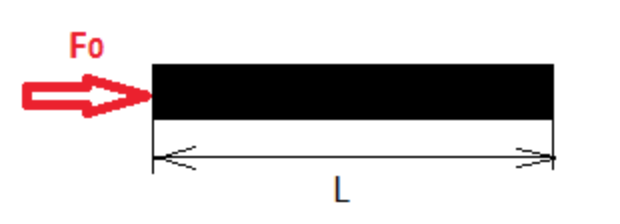
\includegraphics[scale = 0.7]{stick.png}}
		\end{center}
		\caption{Стержень нагревают с одного из торцов}
		\label{stick}
	\end{figure}
	
	\newpage
	
	\section*{Результаты работы.}
	
	\subsection*{1. Представить разностный аналог краевого условия при $x = l$ и его краткий вывод интегро-интерполяционным методом.}
	
	Проинтегрируем уравнение (7.8) с учетом (7.9) из Лекции №7 на отрезке $[x_{N-\frac{1}{2}}, x_N]$
	
	\[-\int_{x_{N-\frac{1}{2}}}^{x_N}\frac{dF}{dx}dx-\int_{x_{N-\frac{1}{2}}}^{x_N}p(x)u d(x)+\int_{x_{N-\frac{1}{2}}}^{x_N}f(x)dx = 0\]
	
	Второй и третий интегралы вычислим методом трапеций
	
	\[
	-(F_{x_N}-F_{x_{N-\frac{1}{2}}})-\frac{h}{4}(p_{x_{N-\frac{1}{2}}} y_{x_{N-\frac{1}{2}}} + p_{x_N} y_{x_N}) + \frac{h}{4} (f_{x_{N-\frac{1}{2}}} + f_{x_N}) = 0.
	\]
	
	Подставляя выражение для $F_{x_{N-\frac{1}{2}}}$ согласно (7.12) из Лекции №7 при $n = N$ и краевое условие при $x = l$ ($x_N$), придем к формуле
	
	\begin{equation}\label{f1}
		y_N = \frac{
			\chi_{N-\frac{1}{2}}-\frac{h^2}{8}p_{N-\frac{1}{2}}
		}{
		\alpha h + \frac{h^2}{4}p_N+\frac{h^2}{8}p_{N-\frac{1}{2}}+\chi_{N-\frac{1}{2}}
	} y_{N-1} + \frac{
	\frac{h^2}{4}(f_{N-\frac{1}{2}}+f_N)+h\alpha \beta
}{
	\alpha h + \frac{h^2}{4}p_N+\frac{h^2}{8}p_{N-\frac{1}{2}}+\chi_{N-\frac{1}{2}}
}
	\end{equation}
	
	Где $\alpha = \alpha_N, \beta = T_0$
	
	Можно принять простую аппроксимацию
	
	\[p_{N-\frac{1}{2}} = \frac{p_{N-1}+p_N}{2}, f_{N-\frac{1}{2}} = \frac{f_{N-1}+f_N}{2}\]
	
	При уменьшении шага (в пределе при $h\rightarrow0$), в (\ref{f1}) членами, содержащими $h^2$ можно пренебречь, тогда (\ref{f1}) преобразуется к виду
	
	\[
	y_N = \frac{\chi_{N - \frac{1}{2}}}{\alpha h + \chi_{N - \frac{1}{2}}} y_{N-1} + \frac{h \alpha \beta}{\alpha h + \chi_{N-\frac{1}{2}}}
	\]
	
	\newpage
	
	\subsection*{2. График зависимости температуры $T(x)$ от координаты x при заданных выше параметрах.}
	
	Ниже представлен график с шагом 0.01 см; $F_0 = 50$ Вт/см$^2$.
	
	\begin{figure}[h!]
		\begin{center}
			{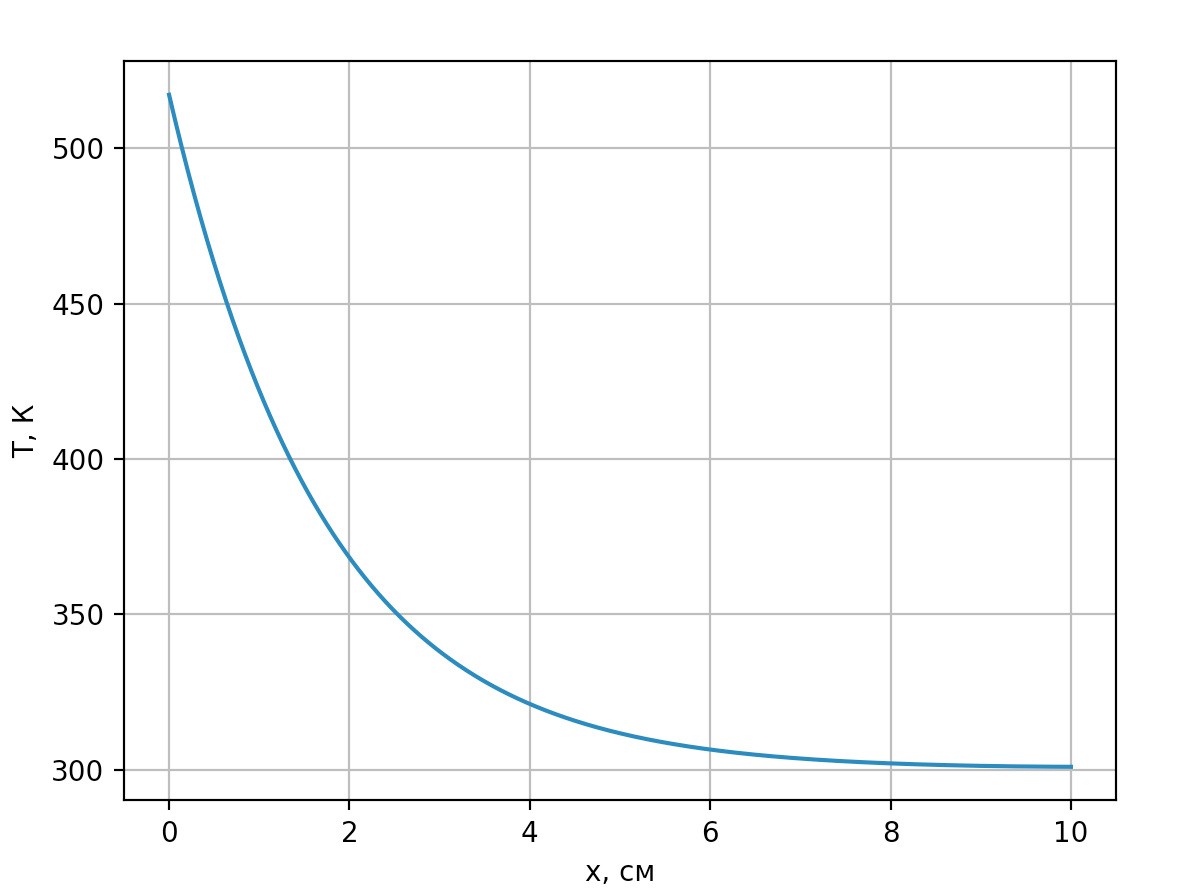
\includegraphics[scale = 0.4]{0.01.png}}
			\label{ris:0.01}
		\end{center}
		\caption{График зависимости температуры $T(x)$ от координаты x при h = 0.01 см; $F_0 = 50$ Вт/см$^2$.}
	\end{figure}

	
	\subsection*{3. График зависимости $T(x)$ при $F_0$ = -10 Вт/см$^2$. }
	
	\begin{center}
		\textit{Справка}. При отрицательном тепловом потоке слева идет съем тепла, поэтому
		производная $T'(x)$ должна быть положительной.
	\end{center}

	Ниже представлен график с шагом 0.01 см; $F_0 = -10$ Вт/см$^2$.

	\begin{figure}[h!]
		\begin{center}
			{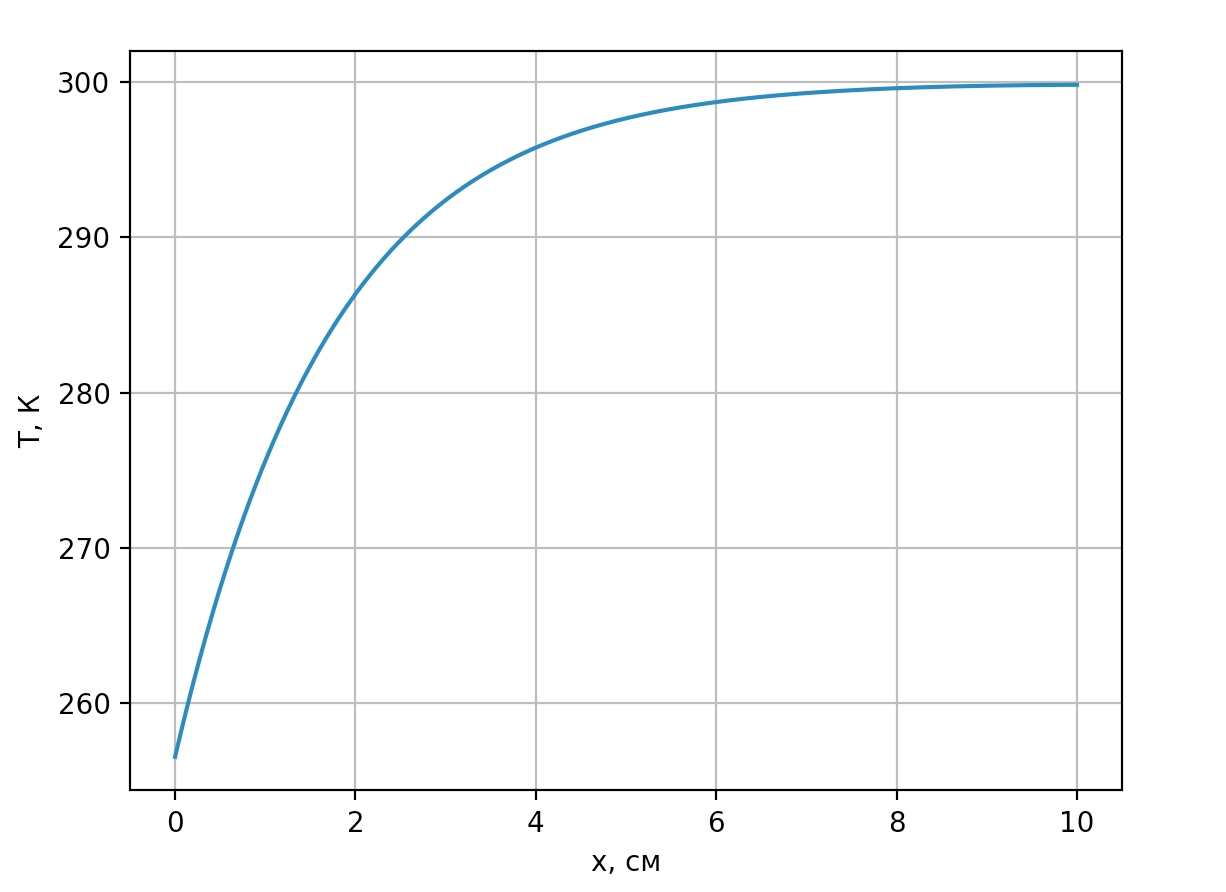
\includegraphics[scale = 0.4]{-10.png}}
			\label{ris:-10}
		\end{center}
		\caption{График зависимости температуры $T(x)$ от координаты x при h = 0.01 см; $F_0 = -10$ Вт/см$^2$.}
	\end{figure}
	
	\newpage
	
	\subsection*{4. График зависимости $T(x)$ при увеличенных значениях $\alpha(x)$ (например, в 3 раза). }
	
	Сравнить с п.2.
	
	\begin{center}
		\textit{Справка}. При увеличении теплосъема и неизменном потоке $F_0$ уровень температур $T(x)$ должен снижаться, а градиент увеличиваться.
	\end{center}

	Ниже представлен график с шагом 0.01 см; $F_0 = 50$ Вт/см$^2$; $\alpha_0$ = 0.15 Вт/см$^2$ К, $\alpha_N$ = 0.03 Вт/см$^2$ К (увеличено в 3 раза).
	
	\begin{figure}[h!]
		\begin{center}
			{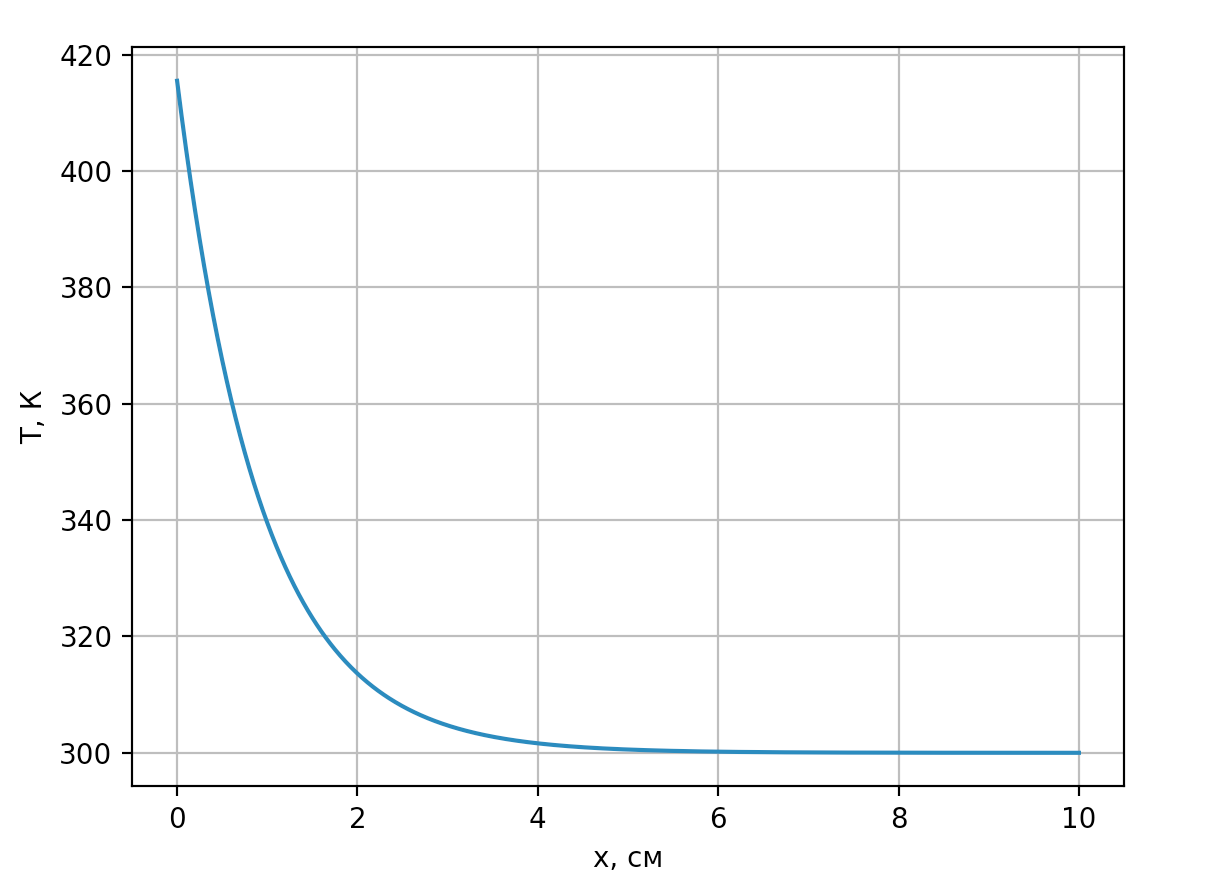
\includegraphics[scale = 0.7]{3.png}}
			\label{ris:3}
		\end{center}
		\caption{График зависимости температуры $T(x)$ от координаты x при h = 0.01 см; $F_0 = 50$ Вт/см$^2$; $\alpha_0$ = 0.15 Вт/см$^2$ К, $\alpha_N$ = 0.03 Вт/см$^2$ К.}
	\end{figure}
	
	\newpage
	
	\subsection*{5. График зависимости $T(x)$ при $F_0 = 0$.}
	
	\begin{center}
		\textit{Справка}. В данных условиях тепловое нагружение отсутствует, причин для
		нагрева нет, температура стержня должна быть равна температуре окружающей
		среды $T_0$
		(разумеется с некоторой погрешностью, определяемой приближенным
		характером вычислений).
	\end{center}

	Ниже представлен график с шагом 0.01 см; $F_0 = 0.0$ Вт/см$^2$.
	
	\begin{figure}[h!]
		\begin{center}
			{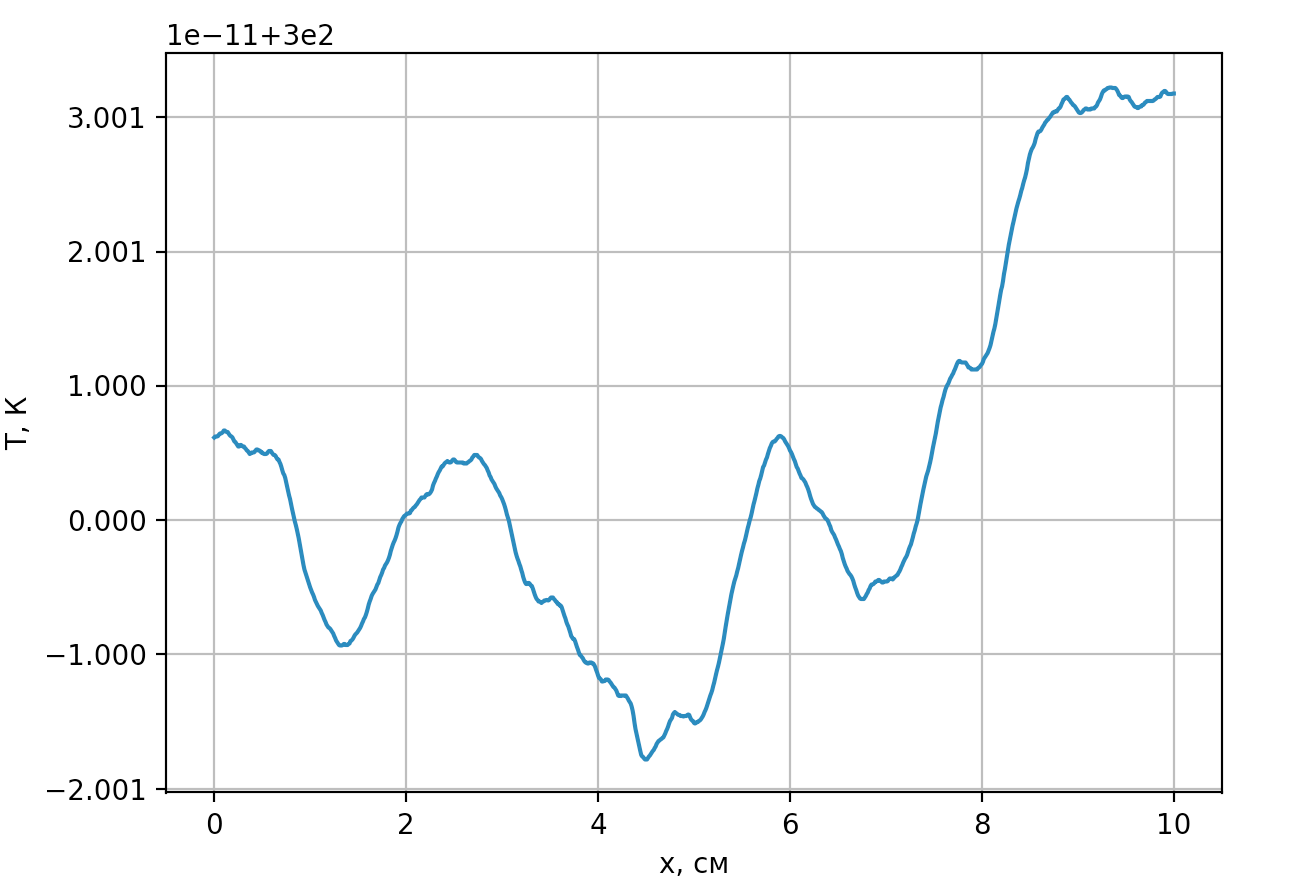
\includegraphics[scale = 0.7]{0.png}}
			\label{ris:0}
		\end{center}
		\caption{График зависимости температуры $T(x)$ от координаты x при h = 0.01 см; $F_0 = 0.0$ Вт/см$^2$.}
	\end{figure}

	\newpage

	\section*{Вопросы при защите лабораторной работы.}
	
	Ответы на вопросы дать письменно в отчете о лабораторной работе.
	
	\subsection*{1. Какие способы тестирования программы можно предложить?}
	
	\begin{enumerate}
		\item Первым делом, необходимо проверить, как будет вести себя график при положительно заданном $F_0$. Физический смысл этого тестирования такой: $F_0$ - тепловой поток, которым нагревают стержень с левого края. Если он больше 0, то температура стержня слева должна быть выше окружающей температуры $T_0$, и чем ближе мы приближаемся к правому краю, с которого нагрева нет (рис. \ref{stick}), тем сильнее график $T(x)$ должен приближаться к значению $T_0$ (см. пункт 2 в Результатах работы).
		\item Аналогично при отрицательных значениях $F_0$ происходит охлаждение стержня с левой стороны, значит значение функции $T(x)$ при $x = 0$ должно быть меньше температуры окружающей среды $T_0$, и затем постепенно (по мере увеличения $x$) приближаться к $T_0$(см. пункт 3 в Результатах работы).
		\item Следующий способ тестирования - увеличение/уменьшение начальных значений $\alpha(x)$: $\alpha_0, \alpha_N$, которые являются коэффициентами теплоотдачи при обдуве, и, соответственно, чем выше эти коэффициенты, тем меньше должен быть уровень температур при неизменном потоке $F_0$ (см. пункт 4 в Результатах работы).
		\item Последний способ: задать $F_0 = 0$. То есть стержень не охлаждается и не нагревается, в следствие чего должна получиться "прямая" линия (с учетом некоторой погрешности) на всем интервале $x\in[0;l]$, принимающая значение $T = 300$К (температура окружающей среды) (см. пункт 5 в Результатах работы).
	\end{enumerate}
	
	\subsection*{2. Получите простейший разностный аналог нелинейного краевого условия при}
	
	\begin{equation}\label{f2}
	x = l, -k(l)\frac{dT}{dx}=\alpha_N(T(L)-T_0)+\varphi(T),
	\end{equation}
	
	где $\varphi(T)$ - заданная функция.
	
	\textit{Решение:}
	
	Аппроксимируя производную  односторонней разностью имеем:
	
	\begin{equation}\label{f5}
	-k_N\frac{y_N - y_{N-1}}{h} = \alpha_N(y_N-T_0) + \varphi(y_N)
	\end{equation}
	

	\subsection*{3. Опишите алгоритм применения метода прогонки, если при x = 0 краевое условие линейное (как в настоящей работе), а при x = l, как в п.2.}
	
	
	Необходимо использовать правую прогонку. В этом случае основаная прогоночная формула записывается в виде
	
	\begin{equation}\label{f3}
	y_n = \xi_{n+1} y_{n+1}+\eta_{n+1},
	\end{equation}
	
	а рекуррентные соотношения для определения прогоночных коэффициентов
	
	 \[\xi_{n+1}=\frac{C_n}{B_n-A_n\xi_n}, \eta_{n+1}=\frac{F_n+A_n\eta_n}{B_n-A_n\xi_n}\]
	 
	 Принимая простейшую (первого порядка точности) аппроксимацию краевого условия $x = 0$, получим его разностный аналог
	 
	 \[-k_0\frac{y_1 - y_0}{h} = F_0\]
	 
	 Откуда, учитывая, что $y_0 = \xi_{1} y_{1}+\eta_{1}$, найдем
	 
	 \[\xi_1 = 1, \eta_1 = \frac{hF_0}{k_0}\]
	 
	 Аналогичная разностная аппроксимация правого краевого условия имеет вид (\ref{f5}).
	 
	 Откуда получаем уравнение для определения $y_N$
	 
	 \begin{equation}\label{f6}
	 \varphi(y_N) + y_N(\alpha_N + \frac{k_N}{h}(1 - \xi_N)) - \alpha_N T_0 - \eta_{N} = 0
	 \end{equation}
	 
	Решение данного уравнения удобно искать, например, методом половинного деления. К этому моменту прогоночные коэффициенты $\xi_N, \eta_N$ уже определены.
	 
	
	
	\subsection*{4. Опишите алгоритм определения единственного значения сеточной функции $y_p$ в одной заданной точке $p$. Использовать встречную прогонку, т.е. комбинацию правой и левой прогонок (лекция №8). Краевые условия линейные.}
	
	\textit{Дано:}
	
	Коэффициенты $A_n, B_n, C_n, F_n$ уравнения $A_n y_{n - 1} - B_n y_n + C_n y_{n + 1} = -F_n$.
	
	Краевые условия линейны, то есть:
	
	\begin{enumerate}
		\item $K_0 y_0 + M_0 y_1 = P_0$
		\item $K_N y_N + M_N y_{N - 1} = P_N$
	\end{enumerate}
	
	
	Алгоритм действий:
	
	\begin{enumerate}
		\item Вычисляем прогоночные коэффициенты правой и левой прогонок по следующим формулам:
		\begin{itemize}
			\item Левая прогонка:
			\begin{enumerate}
				\item $\xi_1 = -\frac{M_0}{K_0}, \xi_{n+1} = \frac{C_n}{B_n-A_n \xi_n}$
				\item $\eta_1 = -\frac{P_0}{K_0}, \eta_{n+1} = \frac{F_n + A_n \eta_n}{B_n-A_n \xi_n}$
			\end{enumerate}
			\item Правая прогонка:
			\begin{enumerate}
				\item $\alpha_N = -\frac{K_N}{M_N}, \alpha_{n-1} = \frac{A_n}{B_n-C_n \alpha_n}$
				\item $\beta_N = -\frac{P_N}{M_N}, \beta_{n-1} = \frac{F_n + C_n \beta_n}{B_n-C_n \alpha_n}$
			\end{enumerate}
		\end{itemize}
		\item Используя рекуррентные соотношения для определения неизвестных $y_i$, составим систему из двух уравнений при $i = p-1$:
		
		\[
		\begin{cases}
		y_{p-1} = \xi_{p} y_{p}+\eta_{p}\\
		y_{p} = \alpha_p y_{p-1} + \beta_{p}
		\end{cases}
		\]
		
		Решая ее, получим:
		
		\[
		y_p = \frac{\alpha_p \eta_p + \beta_p}{1-\alpha_p \xi_p}
		\]
		
		Где коэффициенты $\alpha_p, \eta_p, \beta_p, \xi_p$ уже найдены.
	\end{enumerate}

	\newpage
	
	\section*{Листинг кода программы}
	
	Метод прогоночных коэффициентов:
	
	\begin{figure}[h!]
		\begin{center}
			{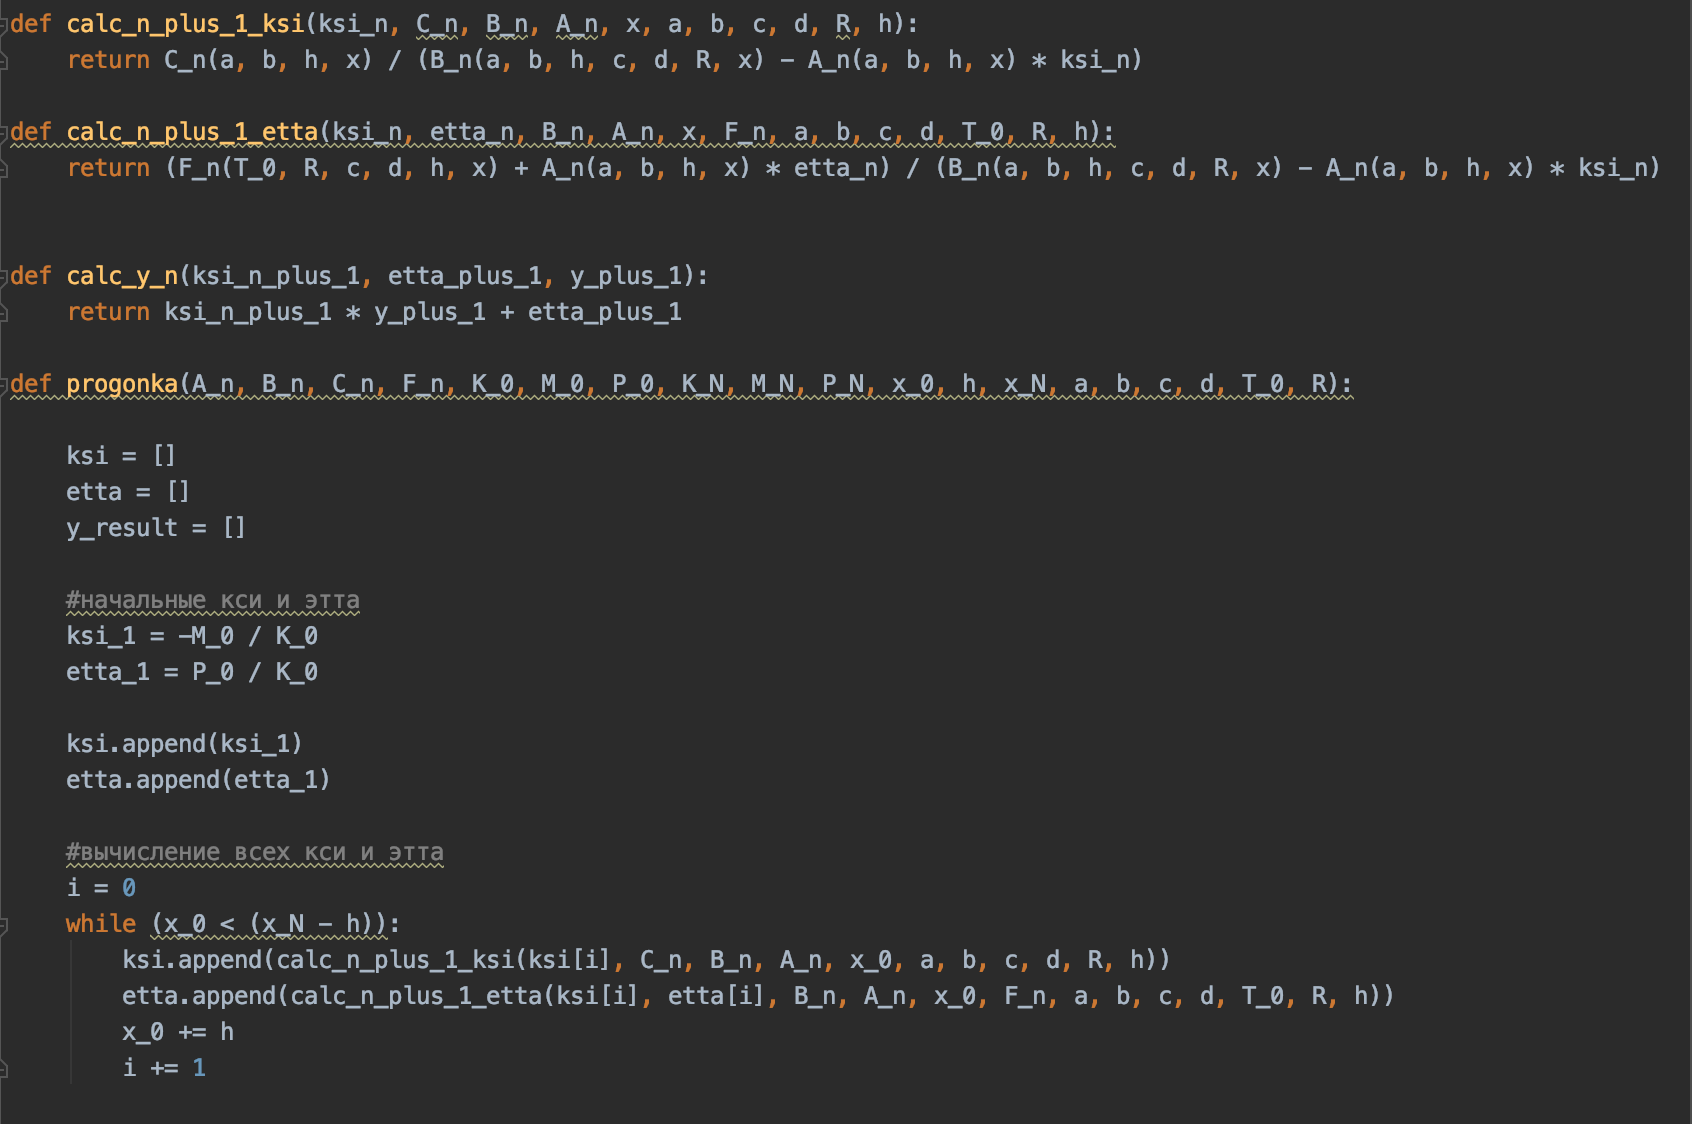
\includegraphics[scale = 0.6]{progonka1.png}}
		\end{center}
		\label{progonka1}
	\end{figure}
	
	\begin{figure}[h!]
		\begin{center}
			{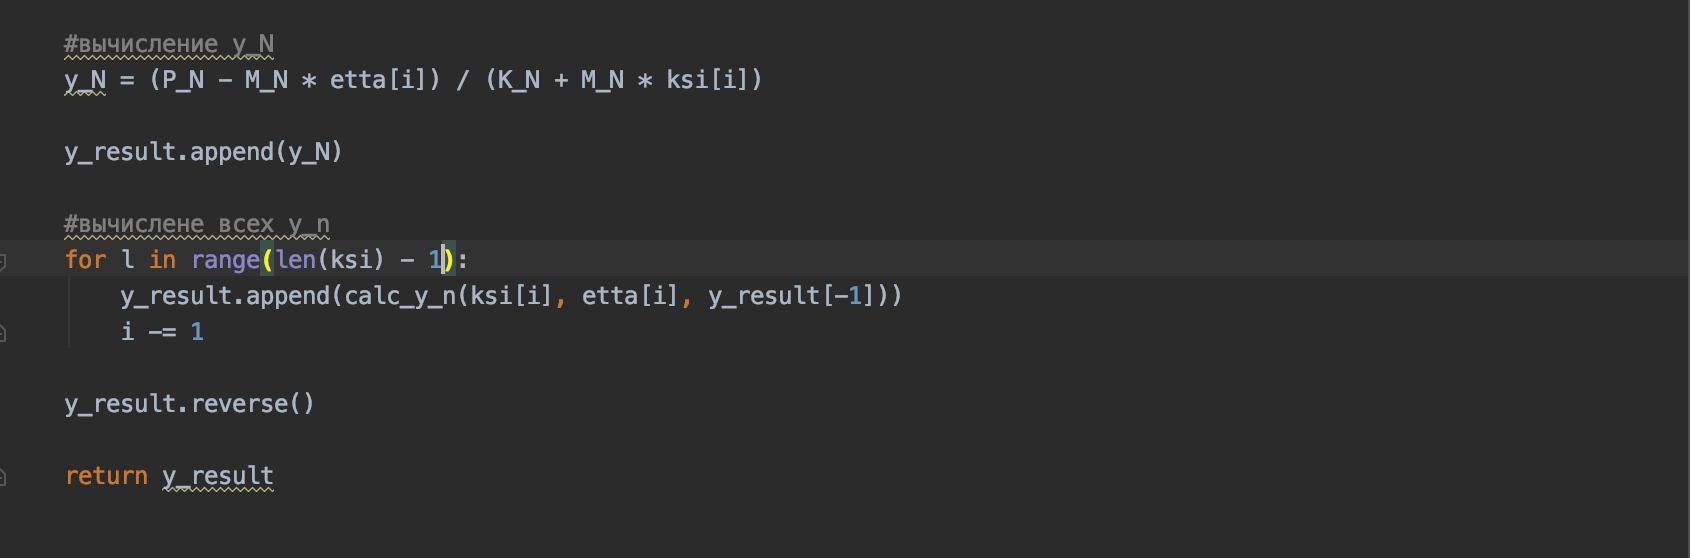
\includegraphics[scale = 0.6]{progonka2.png}}
		\end{center}
		\caption{Реализация метода прогоночных коэффициентов.}
		\label{progonka2}
	\end{figure}

	\newpage
	
	Реализация задачи:
	
	\begin{figure}[h!]
		\begin{center}
			{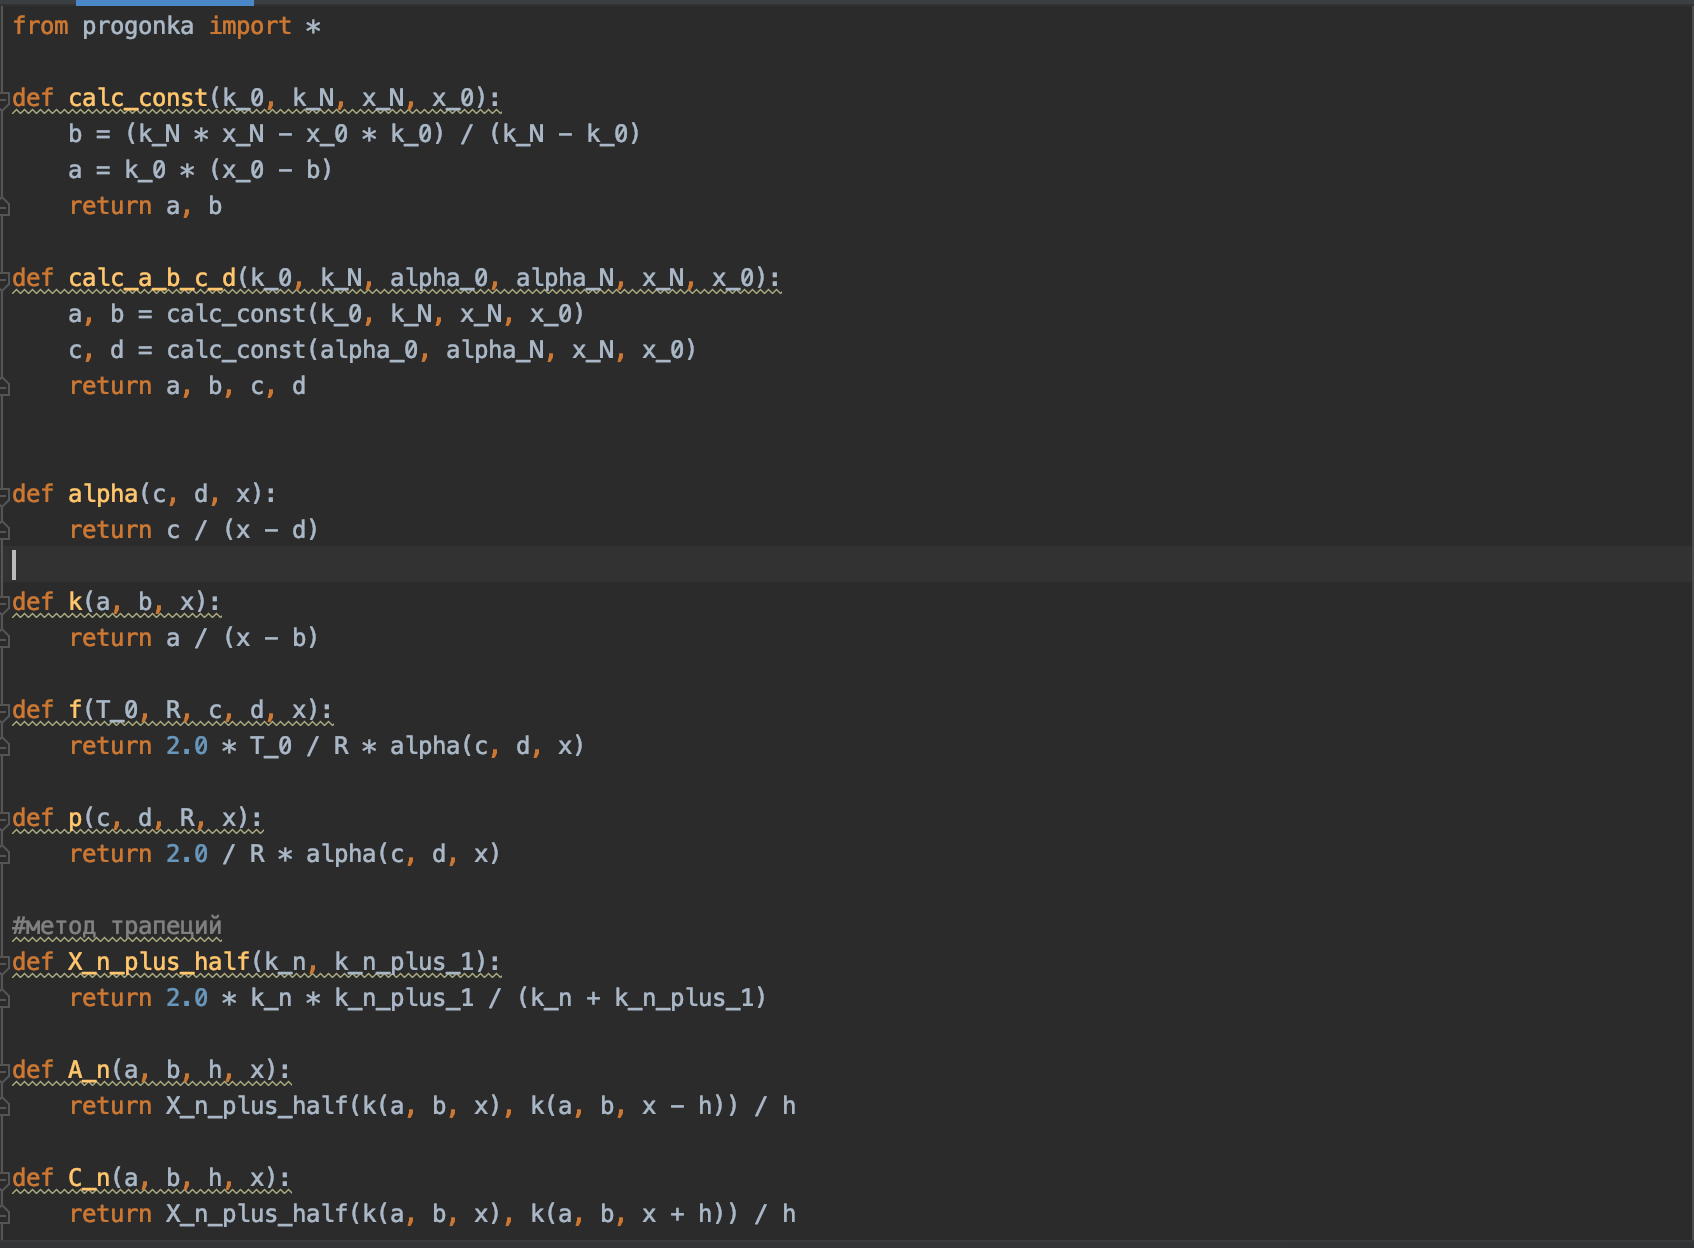
\includegraphics[scale = 0.6]{task1.png}}
		\end{center}
		\label{task1}
	\end{figure}
	
	\begin{figure}[h!]
		\begin{center}
			{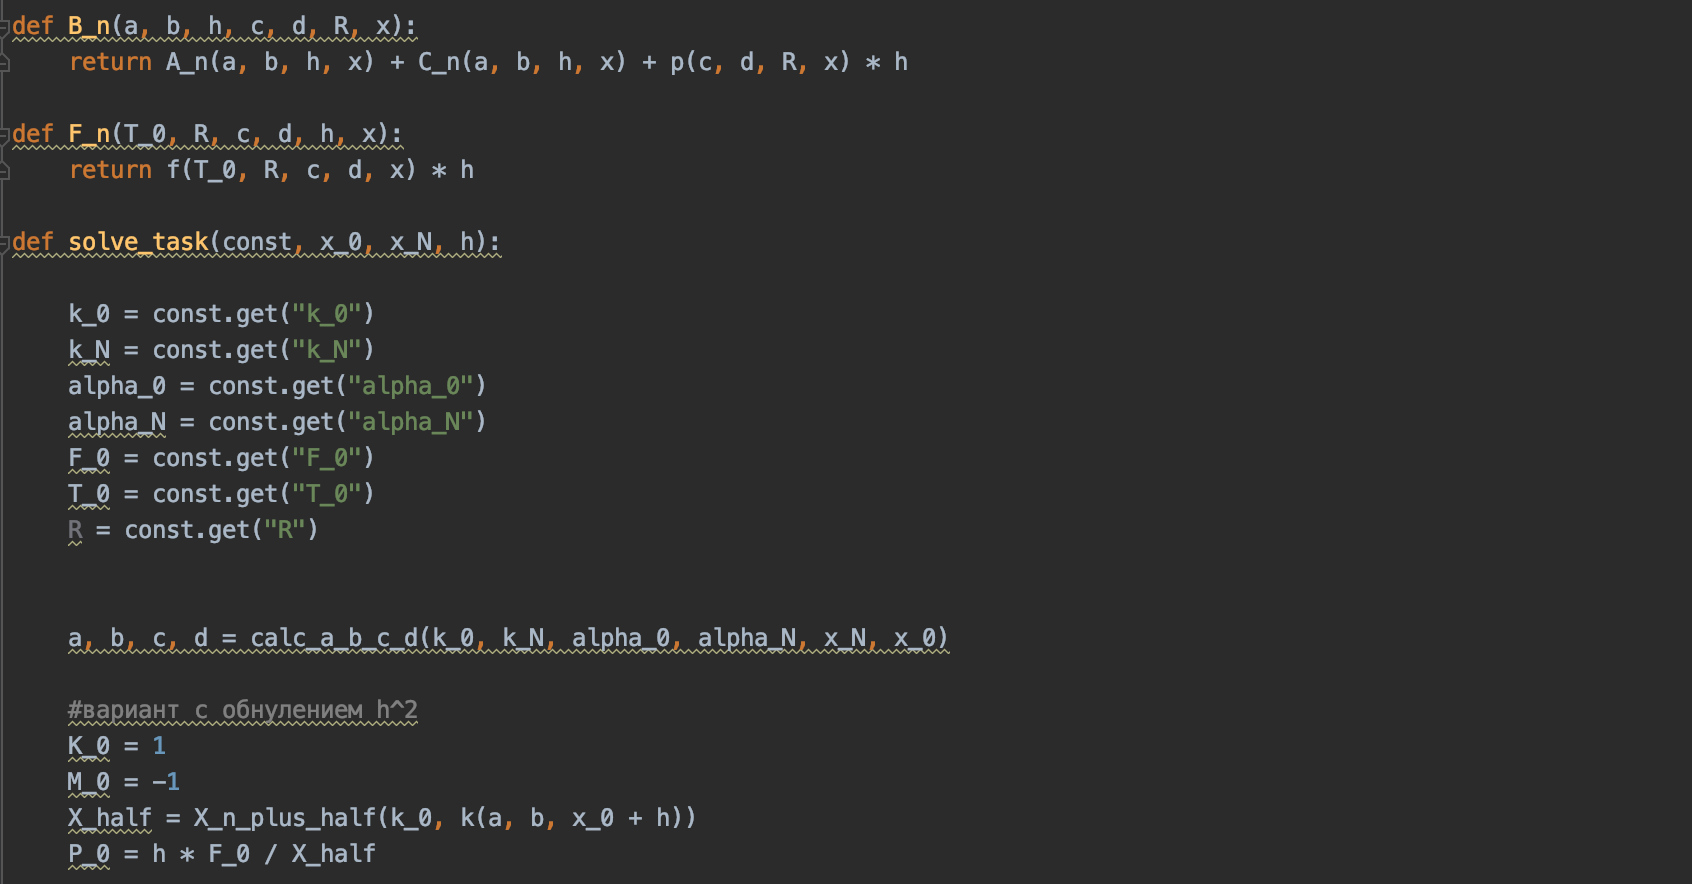
\includegraphics[scale = 0.6]{task2.png}}
		\end{center}
		\label{task2}
	\end{figure}

	\begin{figure}[h!]
		\begin{center}
			{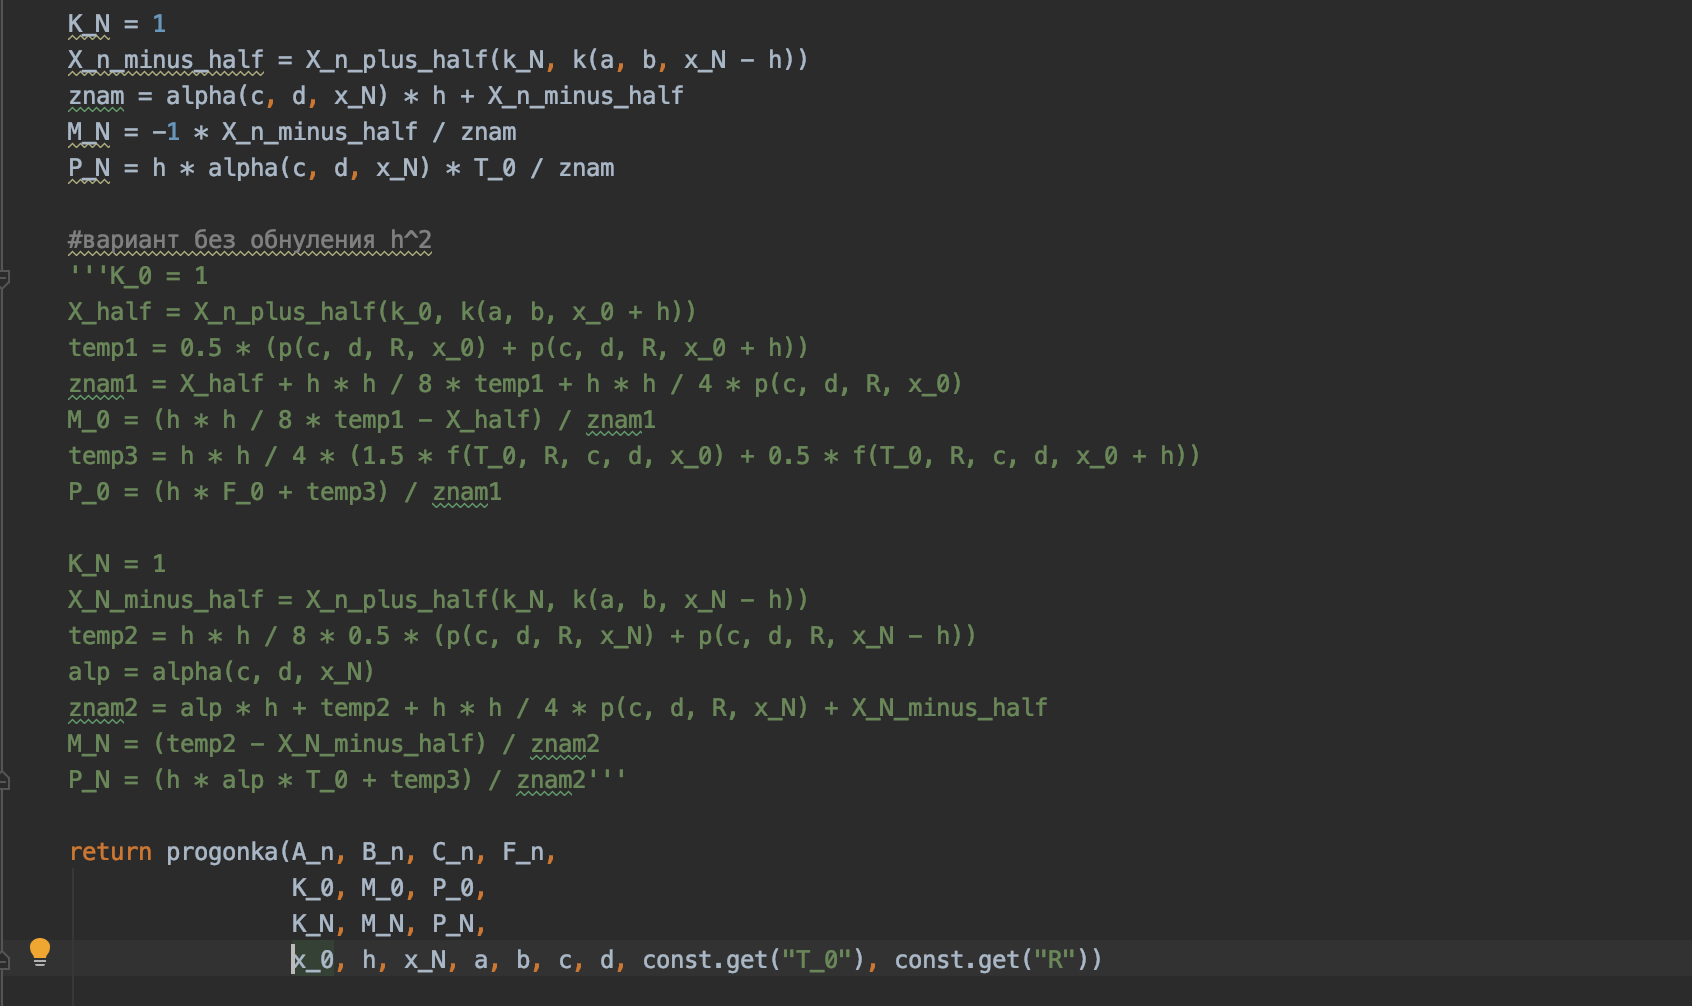
\includegraphics[scale = 0.6]{task3.png}}
		\end{center}
		\caption{Вычисление коэф. a, b, c, d, и коэф. линейных краевых условий}
		\label{task3}
	\end{figure}

	\section*{Интерфейс программы}
	
	\begin{figure}[h!]
		\begin{center}
			\begin{minipage}[h!]{0.5\linewidth}
				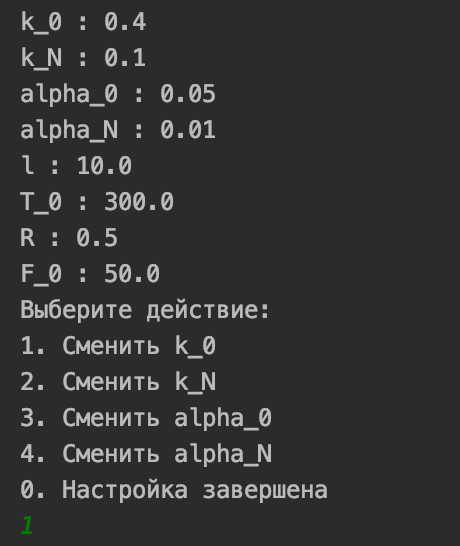
\includegraphics[width=0.9\linewidth]{interf1.png}
			\end{minipage}
			\begin{minipage}[h!]{0.49\linewidth}
				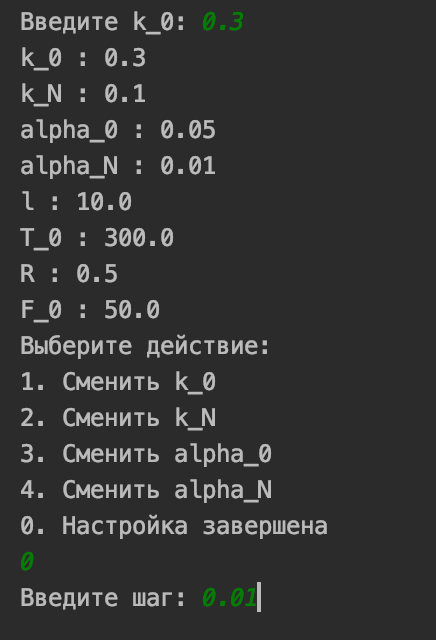
\includegraphics[width=0.75\linewidth]{interf2.png}
			\end{minipage}
		\end{center}
		\caption{Интерфейс программы}
		\label{interf}
	\end{figure}

	
\end{document}